\documentclass[a4paper]{report}

\usepackage[francais]{babel}
\usepackage[utf8x]{inputenc}
\usepackage{hyperref}
\usepackage{appendix}

% Images et figures
\usepackage{graphicx}
\usepackage{float}
\usepackage{geometry}

% CdU
\usepackage{xcolor}
\usepackage[colorinlistoftodos]{todonotes}
\usepackage{enumitem}

% Diagrammes de séquence
\usepackage{tikz}
\usetikzlibrary{arrows, shadows}
\usepackage[underline=true, rounded corners=false]{pgf-umlsd}

% Couleurs de cellules
\usepackage{xcolor, colortbl}

% Police: sans-serif
\renewcommand{\familydefault}{\sfdefault}

% Ajustement horizontal d'une image
\newcommand{\adjustimg}{\ifodd\value{page}\hspace*{\dimexpr\evensidemargin-\oddsidemargin}\else\hspace*{-\dimexpr\evensidemargin-\oddsidemargin}\fi}

% Inclusion d'une image en la centrant sur la page
\newcommand{\centerimg}[2][width=\textwidth]{\makebox[\textwidth]{\adjustimg\includegraphics[#1]{#2}}}

\begin{document}

\title{DevOo}
\author{dragibus}

\maketitle

\tableofcontents


\chapter{Capture des besoins}

\section{Modèle du domaine}

\begin{figure}[h]
    \centering
    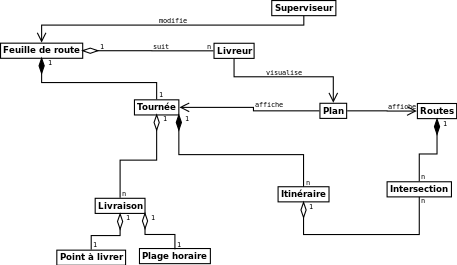
\includegraphics[scale = 0.7]{images/modele-domaine}
    \caption{Modèle du domaine de l'application "OptiFret"}
\end{figure}

\section{Cas d'utilisation}

\subsection{Description textuelle des cas d'utilisation}
~~\\

Description abrégée du cas d'utilisation \textbf{Superviser les tournées}\\

L'utilisateur s'est préalablement identifié sur la plateforme OptiFret, et,
dans le cas d'un Superviseur, la fenêtre de visualisation des feuilles de route
est la première fenêtre apparente. Il pourra parcourir l'ensemble des feuilles
de routes depuis une liste déroulante. Pour chaque feuille de route,
l'utilisateur peut voir la liste des livraisons ordonnée (selon un ordre défini
par le système relatif au trajet à parcourir), dont les informations sont
abrégées. Il peut dérouler chaque livraison pour en avoir les informations
détaillées, puis les enrouler ensuite pour retrouver les informations abrégées.

Il a également accès à differentes informations comme la position GPS du
livreur ou des inforamtions sur livraisons passées (livraison à l'heure ou en
retard, problemes eventuels). \\

Description abrégée du cas d'utilisation \textbf{Modifier feuille de route en
    cours de livraison} \\

Au cas où un changement de l'ordre des livraisons soit nécessaire, le
Superviseur doit avoir la possibilité de modifier les feuilles de route en
temps réel. Cela comprend qu'il peut changer l'ordre des livraisons, ajouter ou
bien supprimer des livraisons dans une feuille de route précisée. Le
Superviseur ne pourra modifier la feuille de route que pour les livraisons non
effectués ni en cours de route. Après chaque modification le système vérifiera
automatiquement l'intégrité de l'ensemble des livraisons pour cette feuille
avant de les rendre visibles pour le livreur concerné.
Si l'intégrité des livraisons ne peut pas être garantie ou bien qu'un
changement de date et d'heure d'autres livraisons est nécessaire, le
Superviseur est notifié tout de suite par le système et la modification n'est
pas enregistrée. Une fois que le Superviseur a confirmé la notification, il
revient à la fenêtre de la modification, sauf que la fenêtre montrera l'état
initial de la feuille de route.  A chaque modification de la feuille de route
(c'est à dire à chaque modification ou suppression d'une livraison), le système
recalcule automatiquement l'itinéraire. \\

Description abrégée du cas d'utilisation \textbf{Modifier feuille de route
    avant le début de livraison} \\

Si le Superviseur veut supprimer une livraison de l'application OptiFret. Il
sélectionne la livraison à supprimer à partir d'une liste de livraisons et
appuie sur le bouton "supprimer". Si le Superviseur s'est trompé il peut
toujours annuler la dernière action en cliquant sur le bouton "Annuler" (dans
le menu Edition).  S'il existe une erreur dans les informations d'une livraison
ou à la demande du client, le Superviseur selectionne une livraison et peut
modifier l'adresse, la date, l'horaire, le téléphone de contact ou encore
l'intitulé de la livraison (en dehors du cadre du prototype). Dans le cas de
l'ajout d'une livraison une boîte de dialogue s'ouvre et permet de saisir la
nouvelle date.  A chaque modification de la feuille de route (c'est à dire à
chaque modification ou suppression d'une livraison), le système recalcule
automatiquement l'itinéraire.\\

Description abrégée du cas d'utilisation \textbf{Afficher liste des
    livraisons}\\

Si le Superviseur en a besoin, il peut aussi commander l'affichage d'une liste
de toutes les livraisons à partir de la fenêtre de la liste des livraisons par
zône géographique. En bas de cette fenêtre, il trouve un bouton "Afficher
toutes les livraisons" qui lui amènera à la liste complète. Une fois affichée,
le Superviseur a la possibilité de chercher une certaine livraison en utilisant
"Ctrl+F" et d'en sélectionner une pour la modifier. S'il clique sur le bouton
"Modifier" de la livraison choisie, le système va lui demander s'il veut
vraiment modifier cette livraison. La confirmation, par conséquent, lui amènera
à la vue de la modification.\\

Description abrégée du cas d'utilisation \textbf{Contacter client}\\

Dans le cas où la génération des feuilles de route de permet pas de placer la
livraison à un client à l'heure prévue initialement, le Superviseur contacte le
client afin de le prévenir et d'obtenir une nouvelle date de livraison. Il
récupère les informations clients à partir de la visualisation des informations
de la livraison et peut alors le contacter soit par téléphone, soit par adresse
électronique. Il peut alors replacer la livraison dans la liste des demandes de
livraisons après avoir modifié la date et l'heure d'arrivée (cas d'utilisation
"Modifier livraison"). L'ajout dans la liste des demandes de livraisons se met
à jour automatiquement par le système OptiFret.\\

\subsection{Diagramme des cas d'utilisation}

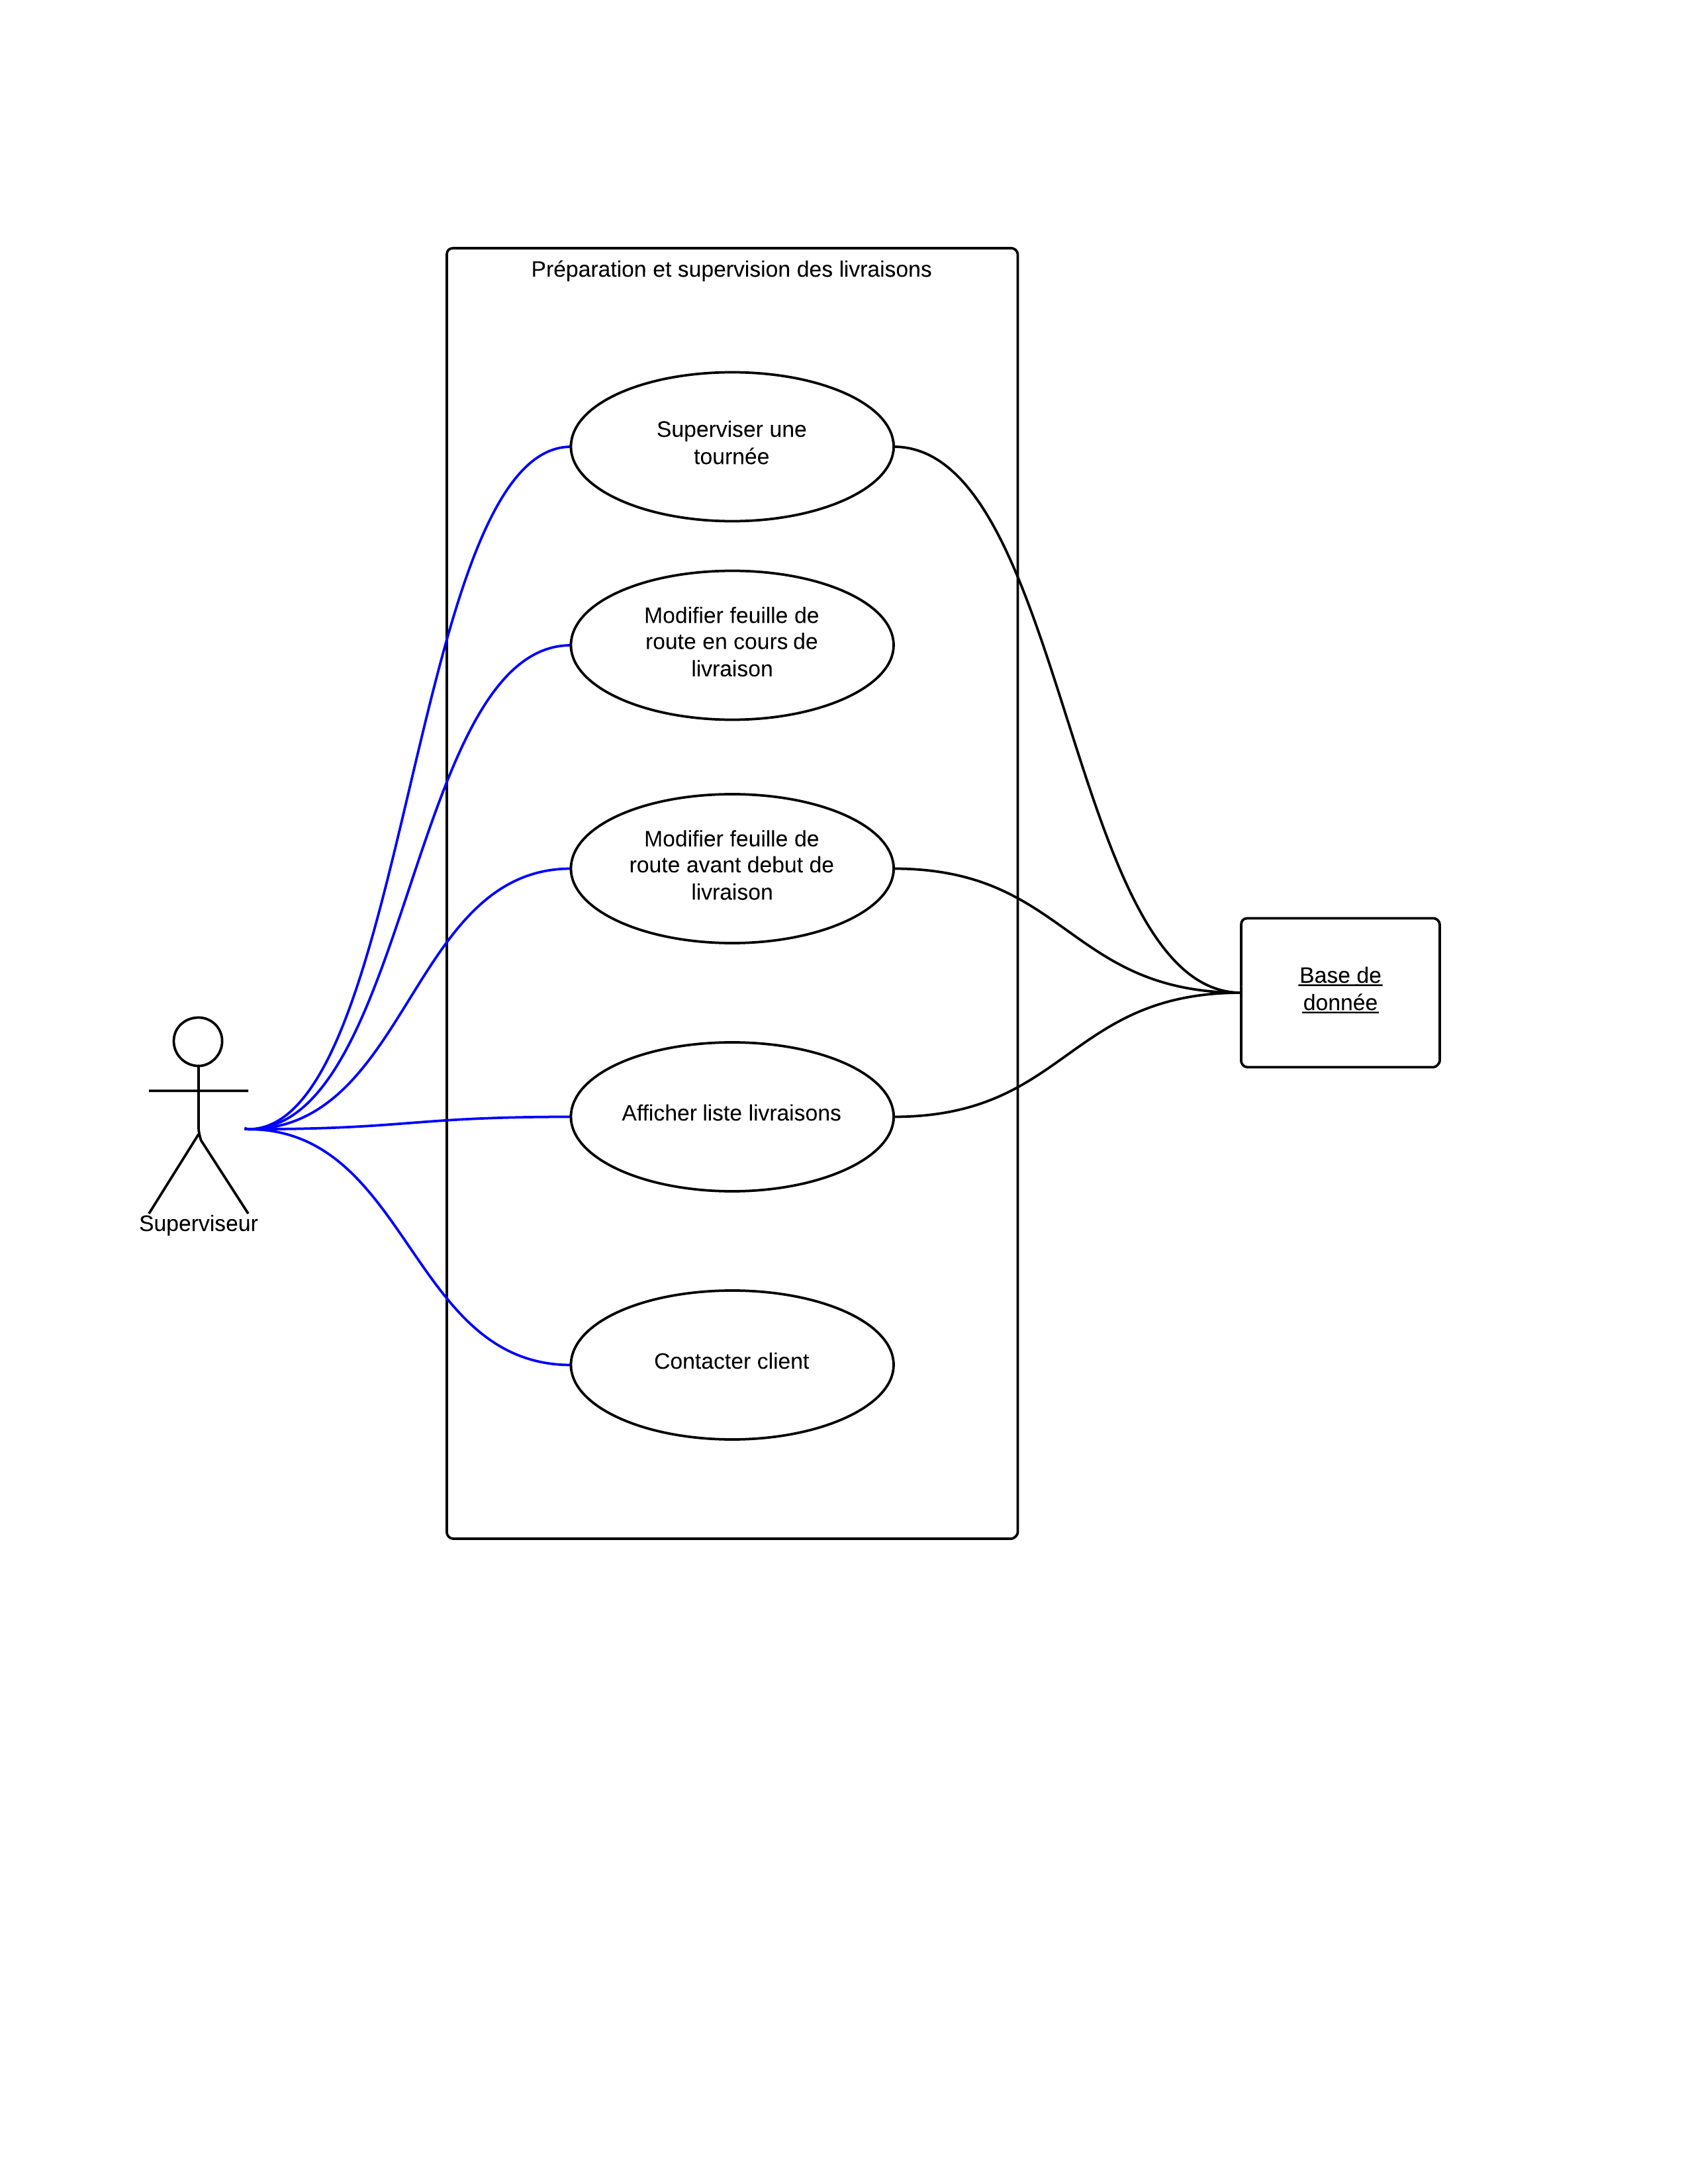
\includegraphics[width=15cm, height=18cm]{images/DiagrammeCdU}

\chapter{Conception}

\section{Description détaillée des cas d'utilisation}

\paragraph{}

Dans cette partie nous abrégerons le terme "cas d'utilisation" par "CdU". \\

\subsection{Visionner les tournées}
\begin{itemize}[label = \textbullet, font = \color{orange}]
    \item \underline{Nom du cas d'utilisation} : visionner les tournées
    \item \underline{Périmètre} : prototype OptiFret
    \item \underline{Niveau} : but utilisateur
    \item \underline{Acteur Principal} : Superviseur
    \item \underline{Parties prenantes et intérêts} :
    \begin{itemize}[label = \textbullet, font = \color{blue}]
        \item \underline{Le Superviseur} : il veut pouvoir visualiser l'état detaillé d'une tournée.
    \end{itemize}
    \item \underline{Préconditions} : L'utilisateur doit être identifié, le plan et la demande de livraisons chargés.
    \item \underline{Postconditions} : Néant.
    \item \underline{Cas Nominal} :
    \begin{enumerate}
        \item La fenêtre de supervision s'affiche dès le Superviseur identifié.
        \item La visualisation d'une tournée s'affiche (détails des livraisons
            et carte avec position du livreur).
        \item En cliquant sur un bandeau de livraison, le Superviseur a accès
            au détails concernant la livraison.
        \item En re-cliquant sur ce bandeau, le Superviseur peut ré-enrouler
            les détails de livraisons pour les masquer.
        \item En cliquant sur une  livraison sur la carte, le Superviseur
            sélectionne la livraison correspondante dans la liste.
        \item Inversement, en sélectionnant une livraison dans la liste, le
            Superviseur peut voir le point de livraison s'afficher sur la
            carte.
    \end{enumerate}
    \item \underline{Extensions} :
    \begin{enumerate}
        \item Aucune carte n'a été chargée : un message d'erreur s'affiche en
            lieu et place de la carte.
        \item Aucune tournée n'est en cours : le menu déroulant est vide.
    \end{enumerate}
    \item \underline{Spécifications particulières} :
    \begin{itemize}[label = \textbullet, font = \color{blue}]
        \item La carte doit être actualisée fréquemment
    \end{itemize}
    \item \underline{Fréquence d'occurence} : très fréquente
    \item \underline{Divers} : Néant.
\end{itemize}

\subsection{Modifier une feuille de route avant le début de livraison}
\begin{itemize}[label = \textbullet, font = \color{orange}]
    \item \underline{Nom du cas d'utilisation} : Modifier une feuille de route
        avant le début de livraison
    \item \underline{Périmètre} : prototype OptiFret
    \item \underline{Niveau} : but utilisateur
    \item \underline{Acteur Principal} : Superviseur
    \item \underline{Parties prenantes et intérêts} :
    \begin{itemize}[label = \textbullet, font = \color{blue}]
        \item \underline{Le Superviseur} : il veut modifier ou supprimer une
            livraison
    \end{itemize}
    \item \underline{Préconditions} : le Superviseur est identifié et
        authentifié sur le système, la feuille de route est chargée sur le
        système, il existe au moins un fichier XML pour une demande de
        livraison et un fichier pour un plan géographique.
    \item \underline{Postconditions} : les modifications sont enregistrés en
        version texte et accessible pour le Livreur concerné
    \item \underline{Cas Nominal} :
    \begin{enumerate}
        \item Le Superviseur se retrouve sur la vue qui affiche les feuilles de
            routes.
        \item Dans le menu "Fichier" il clique sur "Charger un plan" ce qui
            correspond au cas d'utilisation "Charger un plan". Cela sera la
            seule option dans le menu qui est cliquable pour l'instant. Ceci
            correspond au CdU "Charger un plan", visible ci-dessous.
        \item Dans un deuxième temps, il va encore une fois dans le menu
            "Fichier". Maintenant l'option "Charger une demande de livraison"
            est activée aussi. Le Superviseur clique là-dessus pour charger une
            demande de livraisons ce qui correspond au CdU "Charger une
            demande", visible ci-dessous..
        \item La vue lui affiche maintenant la liste des livraisons, ainsi
            qu'un plan de la zone concernée. En plus, les boutons "Supprimer"et
            "Ajouter" (au-dessous du plan) seront activées.
        \item S'il clique sur un point sur le plan qui est déjà inclu dans le
            chemin, le bouton "Ajouter" est désactivé, le bouton "Supprimer"
            reste cliquable. Il en est de même s'il sélectionne une livraison
            dans la liste.
        \item S'il choisit un point non-inclu, le bouton "Ajouter" reste activé
            et le bouton "Supprimer" devient gris et non-cliquable.
        \item Le Superviseur sélectionne une livraison de la liste et clique
            sur le bouton "Supprimer". La dite livraison est retirée de la
            tournée, et du chemin indiqué sur le plan. L'itinéraire est
            automatiquement recalculé.
        \item Il choisit un point du plan, puis il clique sur le bouton
            "Ajouter". Un formulaire apparaît, permettant de compléter les
            informations à propos de cette nouvelle livraison.
        \item Le Superviseur donne donc sa tranche horaire à la nouvelle
            livraison. Elle se retrouve alors dans la tournée.L'itinéraire sera
            alors automatiquement recalculé.
        \item Une fois l'itinéraire calculé, les livraisons de la tournée sont
            marquées d'un code couleur ainsi que les points de livraisons sur
            le plan:
        \begin{itemize}
            \item Vert pour les livraisons qui entrent dans la tournée sans
                aucun problème.
            \item Rouge pour celles qui ne peuvent pas être réalisées dans
                leurs créneaux ou bien qui sont en dehors du temps de travail.
            \item Un dégradé des deux couleurs correspondant au pourcentage du
                temps restant pour respecter le créneau prevu.
        \end{itemize}
        \item En suite, le Superviseur peut recommencer soit à partir du point
            2 soit à partir du point 3.
    \end{enumerate}
    \item \underline{Extensions} : Néant.
    \item \underline{Spécifications particulières} : Néant.
    \item \underline{Fréquence d'occurence} : potentiellement plusieurs fois
        par jour par feuille de route
    \item \underline{Divers} : Néant.
\end{itemize}

\subsection{Charger le plan}
\begin{itemize}[label = \textbullet, font = \color{orange}]
    \item \underline{Nom du cas d'utilisation} : Charger le plan
    \item \underline{Périmètre} : prototype OptiFret
    \item \underline{Niveau} : but utilisateur
    \item \underline{Acteur Principal} : Superviseur
    \item \underline{Parties prenantes et intérêts} :
    \begin{itemize}[label = \textbullet, font = \color{blue}]
        \item \underline{Le Superviseur} : il veut charger le plan
    \end{itemize}
    \item \underline{Préconditions} : le Superviseur est identifié et
        authentifié sur le système
    \item \underline{Postconditions} : la carte est chargée en mémoire (ou non,
        si l'action a été annulée)
    \item \underline{Cas Nominal} :
        \begin{enumerate}
            \item Le Superviseur se retrouve sur la vue qui affiche les
                feuilles de routes.
            \item Il sélectionne dans le menu "Fichier" l'action "Charger le
                plan".
            \item Une nouvelle fenêtre s'ouvre pour choisir un fichier XML.
                Tous les autres types de fichiers ne sonts pas choisissables.
            \item Il sélectionne un fichier XML correspondant à un plan et
                confirme son choix.
            \item Le fenêtre se ferme et il retourne sur la vue d'affichage.
        \end{enumerate}
    \item \underline{Extensions} :
    \begin{enumerate}
        \item Le Superviseur essaye de charger un fichier "invalide"
        \begin{enumerate}
            \item Le système refuse le chargement, et affiche un message
                d'erreur ("Fichier invalide").
        \end{enumerate}
    \end{enumerate}
    \item \underline{Spécifications particulières} : Néant.
    \item \underline{Fréquence d'occurence} : potentiellement plusieurs fois
        par jour
    \item \underline{Divers} : Néant.
\end{itemize}

\subsection{Charger une demande de livraison}
\begin{itemize}[label = \textbullet, font = \color{orange}]
    \item \underline{Nom du cas d'utilisation} : Charger une demande de
        livraison
    \item \underline{Périmètre} : prototype OptiFret
    \item \underline{Niveau} : but utilisateur
    \item \underline{Acteur Principal} : Superviseur
    \item \underline{Parties prenantes et intérêts} :
    \begin{itemize}[label = \textbullet, font = \color{blue}]
        \item \underline{Le Superviseur} : il veut charger une demande de
            livraisons.
    \end{itemize}
    \item \underline{Préconditions} : le Superviseur est identifié et
        authentifié sur le système, le plan a été chargé.
    \item \underline{Postconditions} : les demandes de livraisons sont chargées
        en mémoire (ou non, si l'action a été annulée)
    \item \underline{Cas Nominal} :
    \begin{enumerate}
        \item Le Superviseur se retrouve sur la vue qui affiche les feuilles de
            routes.
        \item Il sélectionne l'action "Charger une demande de livraison" dans
            le menu "Fichier".
        \item Une nouvelle fenêtre pour choisir un fichier XML s'ouvre.
        \item Il sélectionne un fichier XML correspondant à une demande de
            livraison et confirme l'action, tous les autres types de fichiers
            ne sont pas choisissable.
        \item La fenêtre se ferme et il retourne sur la vue d'affichage.
    \end{enumerate}
    \item \underline{Extensions} :
    \begin{enumerate}
        \item Le Superviseur essaye de charger un fichier "invalide"
            \begin{enumerate}
                \item Le système refuse le chargement, et affiche un message
                    d'erreur ("Fichier invalide").
            \end{enumerate}
    \end{enumerate}
    \item \underline{Spécifications particulières} : Néant.
    \item \underline{Fréquence d'occurence} : potentiellement plusieurs fois
        par jour
    \item \underline{Divers} : Néant.
\end{itemize}

\pagebreak

\section{Diagrammes de packages et de classes}

\subsection{Conception initiale}

\begin{figure}[H]
    \noindent\centerimg[width=\paperwidth, height=500pt]{images/ClassDiagram}
    \caption{Diagramme global}
\end{figure}

\begin{figure}[H]
    \noindent\centerimg[width=\paperwidth, height=700pt]{images/model}
    \caption{Diagramme du package modèle}
\end{figure}

\begin{figure}[H]
    \noindent\centerimg{images/controller}
    \caption{Diagramme du package contrôleur}
\end{figure}

\begin{figure}[H]
    \noindent\centerimg{images/view}
    \caption{Diagramme du package vue}
\end{figure}

\subsection{Conception finale}

\begin{figure}[H]
    \noindent\centerimg[width=\paperwidth, height=500pt]{images/fullFinal}
    \caption{Diagramme global final}
\end{figure}

\begin{figure}[H]
    \noindent\centerimg[width=\paperwidth, height=700pt]{images/modelFinal}
    \caption{Diagramme final du package modèle}
\end{figure}

\begin{figure}[H]
    \noindent\centerimg{images/controllerFinal}
    \caption{Diagramme final du package contrôleur}
\end{figure}

\begin{figure}[H]
    \noindent\centerimg{images/viewFinal}
    \caption{Diagramme final du package vue}
\end{figure}

\begin{figure}[H]
    \noindent\centerimg{images/tspFinal}
    \caption{Diagramme final du package config, non prévu initialement}
\end{figure}

\begin{figure}[H]
    \noindent\centerimg{images/configFinal}
    \caption{Diagramme final du package config, non prévu initialement}
\end{figure}

\subsection{Remarques}

Comme on peut le remarquer, la conception a beaucoup changé au cours du
développement, principalement à cause du manque d'idées sur l'interface au
début du projet, ce qui nous a limité en terme de conception. On peut notamment
remarquer que le package \emph{view} a beaucoup changé, et c'est une
conséquence directe du manque d'idées au début du projet. \\

On a aussi vu l'émergence de deux packages non prévus initialement, le package
\emph{tsp} étant une simple encapsulation de toute l'algorithmie concernant le
voyage du commerce. Le package \emph{config} étant dû à la nécessité de
rapidement tester les fonctionnalités de la carte des livraisons, sans avoir à
chaque fois à recharger un fichier XML. \\

Cette configuration a aussi permis de régler les facteurs de zoom et de scroll
dans la carte des livraisons, et a été conçue de telle sorte à ce qu'on puisse
rajouter une configuration dynamique à n'importe quel endroit de l'application,
sans affecter le reste de l'application. Ceci se fait surtout grâce à
l'utilisation d'un accés global en lecture seule de la configuration, via un
design pattern \textbf{Singleton}. \\

Une remarque importante sur l'architecture de l'application: nous considérons
qu'elle ne respecte pas réellement le design pattern MVC, prévu à l'état
initial de la conception. Nous aurions souhaité utiliser un design pattern
\textbf{Observer} entre les modèles et leurs vues, pour permettre une mise à
jour automatique des vues sans avoir à utiliser le contrôleur. Nous n'avons
malheureusement pas eu le temps de mettre cette idée en pratique, vu qu'elle
casserait la totalité de l'application alors qu'il restait encore quelques
fonctionnalités à implémenter rapidement.

\pagebreak

\section{Diagrammes de séquence}

\subsection{Charger les demandes de livraison et calculer la feuille de route}

\begin{figure}[H]
    \begin{sequencediagram}
        \centering
        \newthread{user}{Utilisateur}
        \newinst{lrnListener}{lrn: ActionListener}
        \newinst{ldsListener}{lds: ActionListener}
        \newinst{controller}{:MainController}

        \begin{sdblock}{Chargement d'un plan}{}
            \begin{call}{user}{activate()}{lrnListener}{}
                \begin{call}{lrnListener}{loadRoadNetwork()}{controller}{}
                \end{call}
            \end{call}
        \end{sdblock}

        \begin{sdblock}{Chargement d'une demande de livraison}{}
            \begin{call}{user}{activate()}{ldsListener}{}
                \begin{call}{ldsListener}{loadDeliverySheet()}{controller}{}
                \end{call}
            \end{call}
        \end{sdblock}
    \end{sequencediagram}
\end{figure}

\begin{figure}[H]
    \centering
    \begin{sequencediagram}
        \newthread{controller}{:MainController}
        \newinst{dsModel}{:DeliverySheet}
        \newinst{rnModel}{:RoadNetwork}
        \newinst{dmView}{:DeliveryMap}
        \newinst{dlView}{:DeliveryList}

        \begin{sdblock}{Sélection et chargement d'un XML}{}
            \begin{callself}{controller}{selectFile()}{file}
            \end{callself}
            \begin{call}{controller}{loadFromXML(file)}{rnModel}{}
            \end{call}
        \end{sdblock}
        \begin{sdblock}{Mise à jour des vues}{}
            \begin{call}{controller}{getNodes()}{rnModel}{nodes}
            \end{call}
            \begin{call}{controller}{updateNetwork(nodes)}{dmView}{}
            \end{call}
            \begin{call}{controller}{setDeliveries([])}{dlView}{}
            \end{call}
        \end{sdblock}
    \end{sequencediagram}
    \caption{Détail du diagramme de séquence "charger un plan"}
\end{figure}

\begin{figure}[H]
    \centering
    \begin{sequencediagram}
        \newthread{controller}{:MainController}
        \newinst{dsModel}{:DeliverySheet}
        \newinst{rnModel}{:RoadNetwork}
        \newinst{dmView}{:DeliveryMap}
        \newinst{dlView}{:DeliveryList}

        \begin{sdblock}{Sélection et chargement d'un XML}{}
            \begin{callself}{controller}{selectFile()}{file}
            \end{callself}
            \begin{call}{controller}{loadFromXML(file)}{dsModel}{}
            \end{call}
        \end{sdblock}

        \begin{call}{controller}{makeRoute()}{rnModel}{success}
        \end{call}
        \begin{sdblock}{Solution trouvée}{if success}
            \begin{call}{controller}{getSortedDeliveries()}{rnModel}{delivs}
            \end{call}
            \begin{call}{controller}{setDelivery(delivs)}{dsModel}{}
            \end{call}
            \begin{call}{controller}{createPredTimeSlot()}{dsModel}{}
            \end{call}
        \end{sdblock}
        \begin{callself}{controller}{updateDeliveryMap()}{}
        \end{callself}
        \begin{call}{controller}{getDeliveries()}{dsModel}{deliveries}
        \end{call}
        \begin{call}{controller}{setDeliveries(deliveries)}{dlView}{}
        \end{call}
    \end{sequencediagram}
    \caption{Détail du diagramme de séquence "charger une demande de livraison"}
\end{figure}

\pagebreak

\subsection{Ajouter une livraison}

\begingroup
    \fontsize{6pt}{7pt}\selectfont
    \centering
    \begin{figure}[H]
        \begin{sequencediagram}
            \centering
            \newthread{user}{Utilisateur}
            \newinst{addListener}{add: ActionListener}
            \newinst{controller}{:MainController}
            \newinst{form}{:CreateDeliveryDialog}
            \newinst{subListener}{ok: ActionListener}
            \newinst{dsModel}{:DeliverySheet}

            \begin{call}{user}{activate()}{addListener}{}
                \begin{call}{addListener}{addDelivery()}{controller}{}
                    \begin{call}{controller}{setVisible(true)}{form}{}
                        \begin{call}{user}{activate}{subListener}{}
                        \end{call}
                        \begin{callself}{form}{validateDelivery()}{}
                        \end{callself}
                        \begin{callself}{form}{setVisible(false)}{}
                        \end{callself}
                    \end{call}
                    \begin{call}{controller}{getDelivery()}{form}{delivery}
                    \end{call}
                    \begin{call}{controller}{addDelivery(delivery)}{dsModel}{}
                    \end{call}
                    \begin{callself}{controller}{makeRoute()}{}
                    \end{callself}
                \end{call}
            \end{call}
        \end{sequencediagram}
    \end{figure}
\endgroup

\chapter{Bilan}

\section{Planning prévisionnel du projet}

\begin{center}
    \begin{tabular}{|c|p{2cm}|p{2cm}|p{2cm}|p{2.3cm}|p{2cm}|}
        \hline
        & \multicolumn{2}{|c|}{S1}  &  S1/S2  &  \multicolumn{2}{|c|}{S2} \\\hline
        & Modèle du domaine & Diagramme / Description des cas d'utilisation &
        Détail des cas d'utilisation & UML packages/classes & Diagrammes de
        Séquence\\\hline
        Mathis & 2,5 & 1 & 1 & 3 & 3\\\hline
        Pierre & 2,5 & 1 & 1 & 6 & 0\\\hline
        Patrizia & 0 & 4 & 5,5 & 0 & 0\\\hline
        Quentin & 0 & 4 & 3 & 0 & 0\\\hline
        Julien & 0 & 4 & 3 & 1 & 3\\\hline
        Sylvain & N/A & N/A & 1 & 3 & 3\\\hline
        \multicolumn{6}{|c|}{}\\\hline
        \textbf{Total} & 5 & 14 & 14,5 & 13 & 9\\\hline
    \end{tabular}
\end{center}

\begin{center}
    \begin{tabular}{|c|p{2cm}|p{2cm}|p{2cm}|p{2.3cm}|p{2cm}|}
        \hline
        & S3 & \multicolumn{3}{|c|}{S3/S4/S5} & \textbf{Total} \\\hline
        & Chargement XML & Calcul VDC & Export format texte & Fonctionnalités
        carte & \\\hline
        Mathis & 1,5 & 0 & 5 & 0 & 17\\\hline
        Pierre & 0 & 5 & 0 & 0 & 15,5\\\hline
        Patrizia & 7,5 & 0 & 5 & 4 & 26\\\hline
        Quentin & 0 & 0 & 0 & 8 & 15\\\hline
        Julien & 0 & 5 & 0 & 0 & 16\\\hline
        Sylvain & 0 & 0 & 0 & 8 & 15\\\hline
        \multicolumn{6}{|c|}{}\\\hline
        \textbf{Total} & 9 & 10 & 10 & 20 & 104,5\\\hline
    \end{tabular}
\end{center}

\section{Planning effectif du projet}

\begin{tabular}{|c|p{2cm}|p{2cm}|p{2cm}|p{2.3cm}|p{2cm}|}
    \hline
    & \multicolumn{2}{|c|}{S1}  & S1/S2 & \multicolumn{2}{|c|}{S2} \\\hline
    & Modèle du domaine & Diagramme / Description de cas d'utilisation & Détail
    des cas d'utilisation & UML packages / classes & Diagrammes de séquences
    \\\hline
    Mathis & 2 & 0 & 0 & 0 & 0 \\\hline
    Pierre & 2 & 1 & 0 & 2 & 0 \\\hline
    Patrizia & 0 & 4 & 5,5 & 0 & 0 \\\hline
    Quentin & 0 & 3,5 & 4 & 0 & 0 \\\hline
    Julien & 0 & 3,5 & 4 & 0 & 3 \\\hline
    Sylvain & 0 & 0 & 0 & 10 & 0 \\\hline
    Jean-Marie & 0 & 0 & 1 & 4 & 5 \\\hline
    \multicolumn{6}{|c|}{} \\\hline
    Total & 4 & 12 & 14,5 & 16 & 8 \\\hline
\end{tabular}
~\\
\begin{tabular}{|c|p{2cm}|p{2cm}|p{1cm}|p{1cm}|p{1.7cm}|p{1cm}|p{1.3cm}|c|}
    \hline
    & \multicolumn{7}{|c|}{S3/S4/S5}  & Total  \\\hline
    & Chargement XML & Controlleur principal & Calcul VDC & Export format texte
    & Vue liste livraisons & Vue carte & Batterie tests &  \\\hline
    Mathis & 5 & 0 & 0 & 0 & 6 & 0 & 8 & 21 \\\hline
    Pierre & 0 & 3 & 11 & 4 & 1 & 2 & 6 & 32 \\\hline
    Patrizia & 7,5 & 1 & 0 & 5 & 0 & 4 & 0 & 27 \\\hline
    Quentin & 0 & 4 & 0 & 0 & 15 & 1 & 0 & 27,5 \\\hline
    Julien & 0 & 0 & 6 & 8 & 2 & 2 & 4 & 32,5 \\\hline
    Sylvain & 0 & 1 & 0 & 0 & 1 & 11 & 1 & 23 \\\hline
    Jean-Marie & 4 & 15 & 0 & 0 & 2 & 3 & 3 & 37 \\\hline
    \multicolumn{9}{|c|}{} \\\hline
    Total & 16,5 & 24 & 17 & 17 & 27 & 23 & 22 & 200 \\\hline
\end{tabular}

\section{Bilan technique et humain}

\subsection{Bilan technique}

La conception s'est principalement déroulée en en utilisant divers outils
collaboratifs de traitement de texte (Google Drive, WriteLaTeX) ou de
modèlisation (LucidChart, Dia, VisualParadigm). \\

Pour mettre en place et garder un œil sur nos tâches, nous avons utilisé la
plateforme \href{https://trello.com/}{Trello}, se basant sur des listes de
tâches. Nos 3 listes de tâches étaient "A faire", "En cours" et "Terminées",
les noms étant explicites. Cette plateforme étant aussi collaborative, nous
étions informés en temps réel de l'avancement des tâches en recevant des
notifications par mail. Ce fut une réelle découverte d'une plateforme
d'organisation de projet très intuitive et utile pour un développement en
extreme-programming. \\

Le développement s'est concentrée autour d'un dépôt Git hébergé
en open-source sur Github, et la méthode de développement visée était un
\emph{Feature Branch Workflow}, c'est à dire qu'à chaque nouvelle
fonctionnalité devant être ajoutée, une branche Git était créée et se voyait
fusionnée seulement lorsque cette fonctionnalité devait être intégrée. Cette
méthode nous a permis de paralléliser au maximum le travail fourni et d'avancer
en même temps sur des zones du projet pourtant très couplées. \\

L'équipe étant d'avantage formée en Java qu'en un autre langage, le choix de
l'environnement de développement a donc suivi. L'importance de l'interface et
l'absence de contraintes de performances était cependant en faveur du
développement d'une application Web en utilisant un des frameworks MVC modernes
(Django, Rails). La version 7 de Java a donc été utilisée pendant de
développement, avec quelques librairies supplémentaires : \\

\begin{itemize}
    \item \textbf{Choco}, pour la programmation par contraintes
    \item \textbf{SwingX}, utilisée en complément de Swing, pour les layouts
    \item \textbf{Ini4j}, pour la configuration de l'application
\end{itemize}

\subsection{Bilan humain}

Dans l'ensemble, l'équipe a apprécié le sujet du projet, nous permettant de
développer pleinement une application proche de l'utilisateur et dont
l'utilisation serait concrète. Nous avons donc pu nous concentrer sur
l'IHM afin de construire quelque chose d'intuitif. Ceci a donc impliqué des
changements de conception pour faciliter certaines actions, non prévues au
départ. \\

L'équipe est assez divisée en ce qui concerne les livrables demandés, notamment
le travail en parallèle proposé avec les diagrammes UML, qui en pratique sont
plus difficiles à comprendre que le code source commenté du projet, au vu de sa
taille raisonnable. Nous n'avons pu nous rendre compte de nos erreurs de
conception qu'au cours du projet, l'UML \emph{masquant} certains détails
d'implémentation.

\begin{appendices}
    \chapter{Glossaire}

    \begin{itemize}[label = \textbullet, font = \color{orange}]
        \item \underline{Système (Définition) :} sera appelé système
            l'application principale, nommée par "OptiFret".
        \item \underline{Prototype :} l'application OptiFret, développée au
            stade de démonstration.
        \item \underline{Utilisateur :} personne utilisant l'application
            OptiFret.
        \item \underline{Superviseur :} désigne tout utilisateur utilisant
            l'interface "supervision". Utilisateur principal de l'application
            OptiFret.
        \item \underline{Livreur :} employé à qui est attribué une feuille de
            route.
        \item \underline{Client (objet) :}  ce terme désigne toute personne
            ayant fait acte de l'envoi ou la réception d'une livraison. Sera
            traduit en anglais par \emph{client}.
        \item \underline{Destinataire :} personne à qui l'entreprise doit
            remettre un colis dans le cadre d'une livraison.
        \item \underline{Livraison (objet) :} Acte planifié de transfert d'un
            bien d'un expéditeur à un destinataire, à partir de la demande de
            livraison  jusqu'à sa réalisation. Sera traduit en anglais par
            \emph{delivery}.
        \item \underline{Demande de livraison (objet) :} Ensemble des
            livraisons restant à planifier (calcul de l'itinéraire,
            attribution à une feuille de route ...). Correspond à l'XML chargé
            par l'application.
        \item \underline{Feuille de route (objet) :} Ensemble des informations
            (carte, horaire) décrivant la journée d'un livreur. Sera traduit en anglais par \emph{delivery sheet}
        \item \underline{Tournée (objet) :} réalisation d'une feuille de route,
            donc correspond à une feuille de route après calcul du trajet.
        \item \underline{Itinéraire (objet) :} chemin défini pour une certaine
            tournée. Correspond à un graphe formé de routes (arcs) et
            d'intersections (noeuds). Cette notion ressemble à la notion de
            tournée, seulement qu'elle ne connaît en aucun cas les livraisons
            associées aux points du trajet.
        \item \underline{Carte de l'itinéraire :} vue de dessus de
            l'itinéraire, le chemin à suivre mis en valeur. Sera traduit en
            anglais par \emph{delivery map}.
        \item \underline{Plage horaire (objet) :} intervalle délimité par deux
            heures (ex: 13h45 - 14h30), servant à classer les livraisons. Sera
            traduit en anglais par \emph{time slot}.
        \item \underline{Liste déroulante :} liste dont l'affichage peut être
            déroulé verticalement et/ou horizontalement. Ceci permet de limiter
            l'affichage "visible", afin de concentrer au même endroit
            l'affichage d'une longue liste.
        \item \underline{Intégrité des livraisons :} notion de validation d'une
            livraison, une livraison étant "intègre" quand aucune de ses
            données ne sont abbhérantes.
    \end{itemize}

    \chapter{Abréviations}
    \begin{itemize}[label = \textbullet, font = \color{orange}]
        \item \underline{GPS :} GeoPositioning System
        \item \underline{CdU :} Cas d'Utilisation
        \item \underline{IHM :} Interface Homme Machine
    \end{itemize}
\end{appendices}

\end{document}
